\documentclass[]{spie}
\renewcommand{\baselinestretch}{1.0}
\usepackage{amsmath,amsfonts,amssymb}
\usepackage{graphicx,booktabs,array,siunitx}
\usepackage{algorithm,algpseudocode}
\usepackage{placeins,capt-of}
\usepackage{tikz}
\usetikzlibrary{arrows.meta,positioning}
\usepackage[colorlinks=true,allcolors=blue]{hyperref}
\graphicspath{{figures/}}
% Generated evidence numbers; no hand transcription.
\newcommand{\AllWins}{30}
\newcommand{\AllTies}{5}
\newcommand{\AllLosses}{10}
\newcommand{\PairCount}{45}
\newcommand{\InstanceCount}{15}
\newcommand{\EqualServiceN}{20}
\newcommand{\EnergyWins}{10}
\newcommand{\EnergyTies}{5}
\newcommand{\EnergyLosses}{5}
\newcommand{\EnergyMedian}{0.25}
\newcommand{\PriorityWins}{19}
\newcommand{\ServiceWins}{20}
\newcommand{\ServiceTies}{20}
\newcommand{\ServiceLosses}{5}
\newcommand{\AgentComplete}{25}
\newcommand{\BasicComplete}{16}
\newcommand{\ExactP}{0.0103759765625}
\newcommand{\PriorityReduction}{49.69}
\newcommand{\CountReduction}{37.62}
\newcommand{\EnergyMean}{2.14}
\newcommand{\EnergyChangeDirection}{reduction}
\newcommand{\EnergyChangeMagnitude}{2.14}
\newcommand{\SameTasksN}{18}
\newcommand{\SameTasksMean}{2.40}
\newcommand{\AgentSeconds}{55.21}
\newcommand{\BasicSeconds}{13.93}
\newcommand{\BasicPriorityMean}{3.62}
\newcommand{\BasicCountMean}{2.24}
\newcommand{\AgentPriorityMean}{1.82}
\newcommand{\AgentCountMean}{1.40}
\newcommand{\SmallWins}{9}
\newcommand{\SmallTies}{4}
\newcommand{\SmallLosses}{2}
\newcommand{\BasicSmallPriorityMean}{1.40}
\newcommand{\BasicSmallCountMean}{0.80}
\newcommand{\BasicSmallConditionalEnergyMean}{31.66}
\newcommand{\AgentSmallPriorityMean}{0.53}
\newcommand{\AgentSmallCountMean}{0.47}
\newcommand{\AgentSmallConditionalEnergyMean}{30.25}
\newcommand{\MediumWins}{11}
\newcommand{\MediumTies}{1}
\newcommand{\MediumLosses}{3}
\newcommand{\BasicMediumPriorityMean}{2.60}
\newcommand{\BasicMediumCountMean}{1.87}
\newcommand{\BasicMediumConditionalEnergyMean}{58.09}
\newcommand{\AgentMediumPriorityMean}{1.20}
\newcommand{\AgentMediumCountMean}{0.87}
\newcommand{\AgentMediumConditionalEnergyMean}{57.80}
\newcommand{\LargeWins}{10}
\newcommand{\LargeTies}{0}
\newcommand{\LargeLosses}{5}
\newcommand{\BasicLargePriorityMean}{6.87}
\newcommand{\BasicLargeCountMean}{4.07}
\newcommand{\BasicLargeConditionalEnergyMean}{168.02}
\newcommand{\AgentLargePriorityMean}{3.73}
\newcommand{\AgentLargeCountMean}{2.87}
\newcommand{\AgentLargeConditionalEnergyMean}{168.56}

\newcommand{\lex}{\mathop{\mathrm{lex}}}
\newcommand{\IntALNS}{IntALNS}
\renewcommand{\keywords}[1]{%
\par\vspace{0.5ex}{\noindent\normalsize\bfseries Keywords}\enspace #1%
\vspace{0.5ex}}
\algrenewcommand{\algorithmicrequire}{\textbf{Input}}
\algrenewcommand{\alglinenumber}[1]{\footnotesize #1.}
\title{IntALNS: Interpretable LLM-Agent-Controlled Adaptive Large Neighborhood Search for Cooperative Marine Monitoring Task Allocation}
\input{authors.tex}
\pagestyle{empty}
\begin{document}
\maketitle
\begin{abstract}
Cooperative marine monitoring requires joint task allocation and visit sequencing under heterogeneous platform capabilities, service-start time windows, and transfer-energy limits. Changing routes alter task insertion opportunities, requiring decisions that respond to the current allocation. We propose Interpretable Agent-Controlled Adaptive Large Neighborhood Search (IntALNS), which uses allocation observations, search-execution feedback, and strategy examples to generate neighborhood controls with explicit decision rationales. The large language model agent determines how search proceeds, while ALNS reconstructs routes, enforces feasibility, and returns execution outcomes for subsequent decisions. Experiments compare IntALNS with an adaptive ALNS baseline on synthetic monitoring instances under the same search budget. Across \PairCount{} conditions, IntALNS reduces mean priority loss by \PriorityReduction\% and increases complete allocations from \BasicComplete{} to \AgentComplete{}. Search trajectories show sustained gains, and a recorded case connects allocation evidence, the agent's rationale, and executed controls. These results show that IntALNS improves the allocation of important monitoring tasks while providing an interpretable link between allocation bottlenecks, agent rationales, and executed search controls.
\end{abstract}
\keywords{cooperative marine monitoring, task allocation, large language model agent, adaptive large neighborhood search, interpretable search control}
\section{Introduction}
\label{sec:intro}
Cooperative marine monitoring assigns spatially dispersed tasks with varied payload requirements to heterogeneous platforms, as in air--sea environmental monitoring.\cite{bi2024} A feasible allocation must match tasks to capabilities, respect service-start time windows, and retain sufficient transfer energy for subsequent visits and return to base. These constraints couple task-to-platform assignment with visit order, requiring allocation and route planning to be considered jointly.\cite{liu2018}

Constrained task allocation requires feasible assignments and coordinated execution.\cite{nunes2017} Auctions coordinate assignments through bids and task bundles,\cite{choi2009} while evolutionary search addresses capability and timing restrictions for heterogeneous surface vehicles.\cite{wang2024} Adaptive large neighborhood search (ALNS) improves routes by removing and reinserting tasks, adapting operator sampling according to past rewards.\cite{ropke2006} These rewards describe which changes have been productive, whereas current task insertability identifies requests that remain difficult to allocate. The two sources of information are complementary and can jointly direct route reconstruction.

Learning-based search relates the evolving solution to neighborhood control. Graph networks have selected removals while an optimization solver repairs routes,\cite{zhou2023} and reinforcement learning has adapted ALNS operators, removal strength, and acceptance settings.\cite{reijnen2024} Building on this state-driven approach, a large language model (LLM) can interpret allocation observations alongside previous actions and outcomes, then propose controls that a route solver executes while enforcing feasibility.

LLMs have been used to generate candidate solutions from previous evaluations,\cite{opro2024} improve executable heuristics through reflective feedback,\cite{reevo2024} and develop scheduling rules that adjust neighborhood weights during search.\cite{ns4s2025} In marine task allocation, the changing relationship between unassigned tasks and platform routes calls for translating allocation difficulties into a search focus and executable neighborhood operations.

We propose IntALNS, Interpretable Agent-Controlled Adaptive Large Neighborhood Search, to generate state-dependent neighborhood controls and explicit rationales from allocation observations, execution history, and strategy examples. The LLM agent interprets the evolving allocation state and directs search, while ALNS reconstructs feasible routes and returns execution feedback. Experiments evaluate allocation quality and search progress on synthetic marine monitoring instances; a recorded case examines the link between the observed state, agent rationale, executed control, and subsequent outcome.

\section{Problem Formulation}
\label{sec:problem}
Consider a known batch of monitoring tasks planned centrally for heterogeneous platforms with deterministic inputs. Each assigned task is executed without interruption by one platform. Task $i\in\mathcal T$ has a location, required payload and operating capabilities $\mathcal R_i$, service-start time window $[e_i,l_i]$, duration $s_i$, and priority $p_i\geq0$. Platform $a\in\mathcal A$ has capabilities $\mathcal C_a$, speed $v_a>0$, transfer-energy rate $\varepsilon_a$ per distance unit, and energy budget $E_a^{\max}$. All platforms depart from a common base, denoted $0$, at time zero.

A solution $S$ comprises an ordered route $\Gamma_a=(i_{a,1},\ldots,i_{a,n_a})$ for each platform and an unassigned task set $U(S)$. Together, the routes and $U(S)$ partition $\mathcal T$, ensuring unique assignment. Each route includes departure from and return to the base, with task-to-platform assignments and visit orders determined jointly.

Feasibility combines capability matching, timing, and transfer energy. Every assigned task requires $\mathcal R_{i_{a,r}}\subseteq\mathcal C_a$. With Euclidean distance $d_{ij}$, travel time is $\tau^a_{ij}=d_{ij}/v_a$. Set $i_{a,0}=0$ and $b_{a,0}=s_0=0$. The service-start time at each visit is
\begin{equation}
 b_{a,r}=\max\{e_{i_{a,r}},\,b_{a,r-1}+s_{i_{a,r-1}}+\tau^a_{i_{a,r-1},i_{a,r}}\},
 \qquad b_{a,r}\leq l_{i_{a,r}}.
 \label{eq:time}
\end{equation}
Early arrivals wait until the window opens; the upper bound constrains service start. The transfer energy for departure, intertask travel, and return is
\begin{equation}
 E_a(\Gamma_a)=\varepsilon_a\left(\sum_{r=1}^{n_a}d_{i_{a,r-1},i_{a,r}}+d_{i_{a,n_a},0}\right)\leq E_a^{\max}.
 \label{eq:energy}
\end{equation}
Empty routes consume zero energy, and waiting and service contribute only to the time calculation.

Solutions are ranked by the fixed three-level lexicographic objective
\begin{equation}
 \min_S^{\lex}(L_1,L_2,L_3),\qquad
 L_1=\sum_{i\in U(S)}p_i,\quad L_2=|U(S)|,\quad L_3=\sum_{a\in\mathcal A}E_a(\Gamma_a).
 \label{eq:objective}
\end{equation}
Minimizing priority loss $L_1$ favors assigning higher-priority tasks. At equal $L_1$, minimizing the unassigned task count $L_2$ favors including more tasks; at equal $L_1$ and $L_2$, minimizing $L_3$ reduces total transfer energy.

\section{The \IntALNS{} Method}
\label{sec:method}
IntALNS couples interpretable LLM-agent decisions with adaptive large neighborhood search. Allocation observations, execution history, and strategy examples inform neighborhood controls and their stated rationales; ALNS reconstructs routes, enforces feasibility, and returns outcomes for subsequent decisions (Fig.~\ref{fig:framework}). The current and historical-best solutions and adaptive search state persist across windows.

\begin{figure}[htbp]
\centering
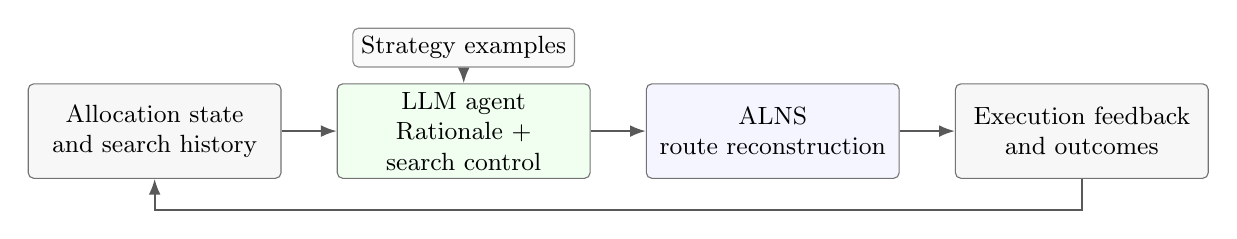
\begin{tikzpicture}[
 box/.style={draw=black!55,rounded corners=2pt,minimum height=12mm,text width=30mm,align=center,font=\small,inner sep=3pt},
 flow/.style={-{Latex[length=2mm]},draw=black!65,line width=.65pt}
]
\node[box,fill=black!3] (state) {Allocation state\\and search history};
\node[box,fill=green!6,right=7mm of state] (agent) {LLM agent\\Rationale +\\search control};
\node[box,fill=blue!4,right=7mm of agent] (solver) {ALNS\\route reconstruction};
\node[box,fill=black!3,right=7mm of solver] (feedback) {Execution feedback\\and outcomes};
\node[draw=black!45,rounded corners=2pt,fill=black!2,above=2mm of agent,font=\small,inner sep=3pt] (examples) {Strategy examples};
\draw[flow] (state)--(agent);
\draw[flow] (examples)--(agent);
\draw[flow] (agent)--(solver);
\draw[flow] (solver)--(feedback);
\draw[flow] (feedback.south)--++(0,-4mm)-| (state.south);
\end{tikzpicture}

\caption{Allocation observations, history, and strategy examples inform LLM rationales and search controls; ALNS executes the controls and returns feedback.}
\label{fig:framework}
\end{figure}

\subsection{Interpretable Search Decisions}
\begin{samepage}
The allocation observation $o_t$ summarizes the search state through current and historical-best objective values, unassigned tasks, compatible platforms, feasible insertion positions, and time and energy margins. The agent uses this information to assess the current allocation and select the search focus and neighborhood controls for the next window.
\par\end{samepage}

\begin{samepage}
At search window $t$, the agent combines $o_t$ with execution history $\mathcal H_t$ and retrieved strategy examples $\mathcal E_t$ to choose $\mathbf u_t$, which specifies the search focus, operator preferences, removal strength, and acceptance setting. The decision is expressed as
\begin{equation}
 \mathbf u_t=\operatorname{LLM}(o_t,\mathcal H_t,\mathcal E_t),
 \label{eq:agent}
\end{equation}
\end{samepage}

Execution history $\mathcal H_t$ records the controls applied in earlier windows together with their observed objective changes, operator use, acceptance outcomes, and insertion results. It supplies the agent with evidence of how previous search adjustments performed and whether allocation progress has continued or stalled. Relating this feedback to the current observation supports decisions about retaining a productive direction, changing operator preferences, or increasing the extent of route reconstruction.

Strategy examples $\mathcal E_t$ are retrieved from development instances according to task scale and search situation. Each example pairs a previous decision with its execution outcome, providing a concrete reference for addressing a related allocation difficulty. The examples broaden the decision context with experience from other searches, while $\mathcal H_t$ supplies feedback from the ongoing run; together, they inform controls suited to the current state.

Interpretability comes from grounding the stated rationale in recorded evidence. For subsequent decisions, the agent must reference actual historical feedback, such as objective changes or insertion results, and explain how it motivates the proposed control. Retaining this rationale alongside the observation, executed control, and subsequent outcome lets readers trace which feedback informed the adjustment and how the stated decision was carried out. This makes the basis of search control explicit.

\subsection{Agent-Controlled Destroy-and-Repair Search}
Within each window, the agent's operator preferences combine with ALNS adaptive weights to select destroy and repair operators. Preferences reflect the current allocation state, while adaptive weights reflect earlier operator performance. Removal strength sets the number of tasks removed; destroy operators select them randomly or by local route cost, spatial proximity, or related time windows.

Removed and previously unassigned tasks form the repair pool. The search focus guides stochastic task selection, either across the pool or toward tasks with limited feasible insertion opportunities. Repair then chooses the feasible position with the smallest incremental transfer energy or samples a feasible position randomly. Reassessing insertion opportunities as routes change allows reconstruction to revise task assignments and visit orders.

Candidates follow the lexicographic objective in Eq.~\eqref{eq:objective}. Improvements in $(L_1,L_2)$ are accepted and deteriorations rejected. At equal $L_1$ and $L_2$, greedy acceptance permits no increase in $L_3$, while threshold or simulated-annealing acceptance can admit temporary increases under the selected setting.\cite{santini2018} The historical-best solution is retained separately from the current solution. Each window's objective changes and search outcomes are added to $\mathcal H_t$ for the next decision. Algorithm~\ref{alg:intalns} summarizes the cycle.

\begin{algorithm}[H]
\caption{IntALNS}
\label{alg:intalns}
\begin{algorithmic}[1]
\Require Instance $I$, feasible initial solution $S_0$, search budget $B$, control interval $h$
\State $S\gets S_0$; $S^\star\gets S_0$; $\mathcal H_0\gets\varnothing$; initialize adaptive search state
\For{$t=0,\ldots,B/h-1$}
  \State Form $o_t$ from $I$, $S$, $S^\star$, insertion opportunities, and remaining budget
  \State Retrieve $\mathcal E_t$; obtain and validate $\mathbf u_t$ using Eq.~\eqref{eq:agent}
  \For{$j=1,\ldots,h$}
    \State Sample operators using $\mathbf u_t$ and adaptive weights; remove and repair tasks to form $S'$
    \State Evaluate $S'$; update $S$ by the acceptance rule, $S^\star$ by Eq.~\eqref{eq:objective}, and search statistics
  \EndFor
  \State Append $\mathbf u_t$ and execution feedback to $\mathcal H_t$ to form $\mathcal H_{t+1}$
\EndFor
\State \Return $S^\star$
\end{algorithmic}
\end{algorithm}

\newpage
\section{Experiments}
\label{sec:experiments}
% Generated full-sample completion and conditional energy statistics.
\newcommand{\SmallEqualServiceN}{10}
\newcommand{\MediumEqualServiceN}{5}
\newcommand{\LargeEqualServiceN}{5}
\newcommand{\SmallEnergyReduction}{4.19}
\newcommand{\BasicSmallComplete}{10}
\newcommand{\AgentSmallComplete}{11}
\newcommand{\MediumEnergyReduction}{0.46}
\newcommand{\BasicMediumComplete}{3}
\newcommand{\AgentMediumComplete}{8}
\newcommand{\LargeEnergyReduction}{-0.27}
\newcommand{\BasicLargeComplete}{3}
\newcommand{\AgentLargeComplete}{6}

% Generated from the selected saved case.
\newcommand{\CaseSize}{100}
\newcommand{\CaseSeed}{6800}
\newcommand{\CaseMaturity}{M50}
\newcommand{\CaseStart}{600}
\newcommand{\CaseFirstTrial}{601}
\newcommand{\CaseEnd}{700}
\newcommand{\CaseStall}{5}
\newcommand{\CaseBeforePriority}{8}
\newcommand{\CaseBeforeCount}{4}
\newcommand{\CaseAfterPriority}{7}
\newcommand{\CaseAfterCount}{3}
\newcommand{\CaseBasicPriority}{1}
\newcommand{\CaseBasicCount}{1}
\newcommand{\CaseFinalCount}{2}
\newcommand{\CaseBeforeRatio}{0.4}
\newcommand{\CaseAfterRatio}{0.5}
\newcommand{\CaseServiceRejections}{87}
\newcommand{\CaseUninsertable}{4}
\newcommand{\CasePreviousTrials}{100}
\newcommand{\CasePlotFirst}{400}
\newcommand{\CasePlotLast}{800}

\subsection{Experimental Environment}
The LLM agent uses DeepSeek-V4-Flash, a mixture-of-experts language model supporting both thinking and non-thinking modes. Experiments disable additional reasoning and set the sampling temperature to 0.

\subsection{Dataset Generation}
Synthetic instances contain six heterogeneous platforms and 50, 100, or 300 tasks, denoted T50, T100, and T300. Task locations, requirements, service durations, time windows, and platform resources are generated jointly from complete, capability-compatible reference routes. The service-start time windows accommodate the reference visits, and energy budgets exceed reference-route transfer energy. Each instance therefore admits a complete feasible allocation. Five instances per scale give \InstanceCount{} instances. Within each instance, one random permutation selects nested task subsets with initial allocation ratios of 10\%, 50\%, and 90\%, denoted M10, M50, and M90. Initial routes preserve the relative order of retained tasks; the remaining tasks are unassigned. Search may reorder or reassign tasks, giving \PairCount{} instance--start conditions.

\subsection{Task Allocation Performance}
Basic is an adaptive ALNS baseline without LLM search control; it updates operator probabilities using historical rewards. Both methods share the initial solutions, operator library, and constraint handling. Basic's parameters were selected on a small separate tuning set, with one configuration per task count. Both methods use algorithm seed 0 and 1200 iters; best solutions are recorded every 100 iters, when IntALNS also updates its controls.

Mean $L_1$ and $L_2$ cover all conditions, and wins/ties/losses (W/T/L) compare IntALNS against Basic under the full lexicographic objective. Mean $L_3$ uses the subset defined in Table~\ref{tab:main}. A complete allocation assigns every task, giving $L_1=L_2=0$.

IntALNS produces solutions with lower priority loss and more complete allocations. Across the \PairCount{} conditions, mean priority loss decreases from \BasicPriorityMean{} to \AgentPriorityMean{}, a reduction of \PriorityReduction\%, while complete allocations increase from \BasicComplete{} for Basic to \AgentComplete{} for IntALNS. Mean unassigned task count also falls, from \BasicCountMean{} to \AgentCountMean{}. Under the full lexicographic objective, IntALNS records \AllWins{} wins, \AllTies{} ties, and \AllLosses{} losses (Table~\ref{tab:main}). The aggregate improvement thus includes both reduced priority loss and fewer omitted tasks.

\begingroup
\setlength{\intextsep}{6pt plus 2pt minus 2pt}
% Generated by scripts/build_evidence.py; do not edit numbers.
\begin{table}[htbp]
\centering
\caption{Final task allocation performance and conditional transfer energy.}
\label{tab:main}
\sisetup{mode=text,detect-weight=true}
\setlength{\tabcolsep}{4pt}
\begin{tabular}{@{}l *{4}{S[table-format=1.2]} *{2}{S[table-format=3.2]} c@{}}\toprule
Size & \multicolumn{2}{c}{Mean $L_1$} & \multicolumn{2}{c}{Mean $L_2$} & \multicolumn{2}{c}{Mean $L_3$ ($\times10^3$)$^{\dagger}$} & W/T/L \\
\cmidrule(lr){2-3}\cmidrule(lr){4-5}\cmidrule(lr){6-7}
 & {Basic} & {IntALNS} & {Basic} & {IntALNS} & {Basic} & {IntALNS} & \\
\midrule
T50 & 1.40 & \bfseries 0.53 & 0.80 & \bfseries 0.47 & 31.66 & \bfseries 30.25 & 9/4/2 \\
T100 & 2.60 & \bfseries 1.20 & 1.87 & \bfseries 0.87 & 58.09 & \bfseries 57.80 & 11/1/3 \\
T300 & 6.87 & \bfseries 3.73 & 4.07 & \bfseries 2.87 & \bfseries 168.02 & 168.56 & 10/0/5 \\
\midrule
All & 3.62 & \bfseries 1.82 & 2.24 & \bfseries 1.40 & 72.36 & \bfseries 71.72 & 30/5/10 \\
\bottomrule\end{tabular}
\par\smallskip\begin{minipage}{\textwidth}\footnotesize
$\dagger$ Mean $L_3$ uses pairs with equal $L_1$ and $L_2$ ($n=10,5,5$ for T50, T100, T300; 20 overall). Displayed energy values are divided by $10^3$. Bold marks lower means.
\end{minipage}
\end{table}

\endgroup

The scale-specific results highlight two aspects of this improvement. T300 has the largest absolute decrease in mean priority loss, from \BasicLargePriorityMean{} to \AgentLargePriorityMean{}, as the same fleet handles the largest task set. At T100, complete allocations increase from \BasicMediumComplete{} to \AgentMediumComplete{} of the 15 conditions, showing that more searches resolve all remaining assignments. Together, these findings indicate better protection of important monitoring tasks and a greater ability to include the full task set in a feasible solution.

The advantage develops at different stages of the search. At T100 and T300, IntALNS reaches lower mean priority loss and unassigned task count by 100 iters and maintains both gaps throughout the search. At T50, IntALNS initially leaves more tasks unassigned, and its advantage emerges later, first in priority loss and then in unassigned task count. These trajectories connect the final allocation gains to improvements developed during search (Fig.~\ref{fig:convergence}).

\begin{figure}[t]
\centering
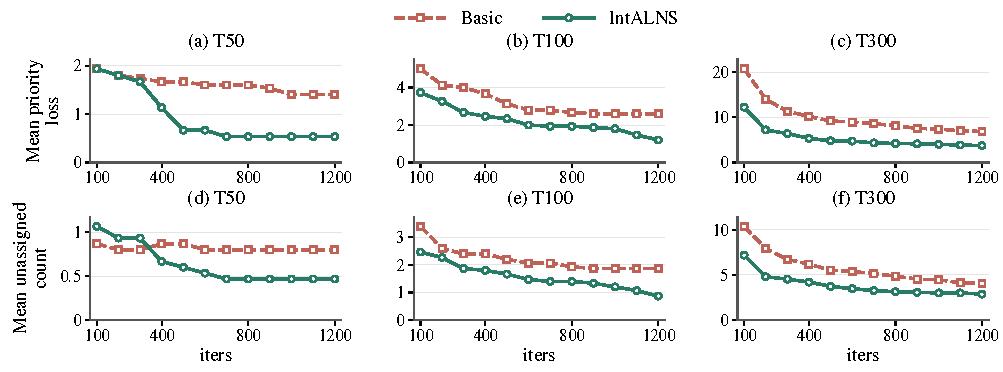
\includegraphics[width=\linewidth]{convergence.pdf}
\caption{Mean priority loss and unassigned task count of the lexicographic-best solutions across the 15 instance--start conditions at each task scale.}
\label{fig:convergence}
\end{figure}

Among pairs with matching $L_1$ and $L_2$, IntALNS achieves lower mean $L_3$ on T50 and T100, whereas T300 shows a small increase (Table~\ref{tab:main}). This increase alone does not indicate poorer allocation performance overall, because equal $L_1$ and $L_2$ can correspond to different task assignments and routes with different transfer-energy costs.

\subsection{Interpretability Analysis}
To examine the interpretability of IntALNS decisions, we trace one search transition from the observed allocation state to the agent rationale, executed control, and subsequent outcome.
At \CaseStart{} iters in T\CaseSize{}, instance \CaseSeed{}, \CaseMaturity{}, $(L_1,L_2)$ had remained unchanged for \CaseStall{} consecutive search windows, while $L_3$ decreased in the latest window. All \CaseUninsertable{} unassigned tasks lacked a feasible insertion position. The agent interpreted this combination as a need to release assigned tasks that blocked further allocation and proposed broader route reconstruction. It increased the removal ratio from \CaseBeforeRatio{} to \CaseAfterRatio{}, keeping the other controls unchanged. The excerpts in Table~\ref{tab:case_decision} link the observed bottleneck to this rationale and the executed control.

By \CaseEnd{} iters, $(L_1,L_2)$ improved from $(\CaseBeforePriority,\CaseBeforeCount)$ to $(\CaseAfterPriority,\CaseAfterCount)$ (Fig.~\ref{fig:case}). The recorded rationale identifies stalled task allocation as the reason for increasing removal strength, making the link between the observed search state and the executed control explicit.

\begin{figure}[H]
\centering
\begin{minipage}[t]{.48\linewidth}
\vspace{0pt}\raggedright
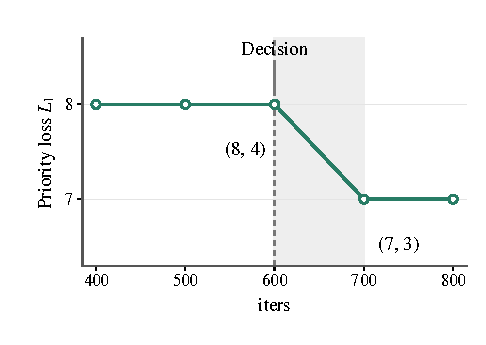
\includegraphics[width=\linewidth]{decision_case.pdf}
\caption{\raggedright Neighborhood adjustment following task-allocation stagnation. Shading marks \CaseStart{}--\CaseEnd{} iters after the control adjustment; labels give $(L_1,L_2)$.}
\label{fig:case}
\end{minipage}\hfill
\begin{minipage}[t]{.48\linewidth}
\vspace{0pt}\raggedright
\captionof{table}{\raggedright Observed bottleneck, decision rationale, and executed control.}
\label{tab:case_decision}
% Generated verbatim field/value and rationale excerpts; provenance in case_raw_excerpt.json.
\begingroup\small\raggedright
\begin{tabular}{@{}>{\raggedright\arraybackslash}p{\linewidth}@{}}
\toprule
\textit{Observed allocation and feedback} \\
\texttt{"zero\_\allowbreak{}feasible\_\allowbreak{}task\_\allowbreak{}count":\nobreakspace 4} \\
\texttt{"consecutive\_\allowbreak{}windows\_\allowbreak{}without\_\allowbreak{}service\_\allowbreak{}progress":\nobreakspace 5} \\
\texttt{"energy\_\allowbreak{}improved\_\allowbreak{}at\_\allowbreak{}equal\_\allowbreak{}service":\nobreakspace true} \\
\midrule
\textit{Agent rationale} \\
``Service has stalled for five windows at [8,4] with all four unassigned tasks showing zero feasible positions, so probe a larger .50 destruction (about 48 tasks) to release coupled assigned blockers'' \\
\midrule
\textit{Executed control} \\
\texttt{"remove\_\allowbreak{}ratio":\nobreakspace 0.5} \\
\texttt{"focus\_\allowbreak{}id":\nobreakspace "service\_\allowbreak{}bottleneck"} \\
\bottomrule
\end{tabular}
\endgroup

\end{minipage}
\end{figure}

\FloatBarrier
\begin{samepage}
\section{Conclusion}
We propose IntALNS for cooperative marine monitoring, formulating task allocation and route sequencing under platform capability, service-start time-window, and transfer-energy constraints. We design an agent-control mechanism that integrates allocation observations, execution history, and strategy examples to guide feasible ALNS route reconstruction. Requiring rationales to cite actual historical feedback makes search adjustments interpretable, as illustrated by the recorded case. Across \PairCount{} synthetic conditions, IntALNS reduces mean priority loss by \PriorityReduction\% and increases complete allocations from \BasicComplete{} to \AgentComplete{} compared with Basic under the same search budget. IntALNS thus combines better allocation of important monitoring tasks with search control grounded in recorded evidence.
\par\end{samepage}

\bibliography{references}
\bibliographystyle{spiebib}
\end{document}
